\documentclass[../writeup.tex]{subfiles}

\begin{document}
\chapter{Latent Semantic Analysis: David Blincoe}\label{chapter:david}
% cite stuff using \autocite{label}, not \cite, for example
% \autocite*{brief-summarization-survey}

% label sections with \label{ch:sec:sectionName}
% and figures with \label{ch:fig:figName},
% equations with \label{ch:eq:eqName}, etc.
% reference labeled stuff with \ref{ch:sec:sectionLabel} to automatically update numbers

% to display something from the images/ directory
% \begin{figure}[h]
%   \centering
%   \includegraphics[width=0.75\textwidth]{image.file}
%   \caption{your caption here}
%   \label{ch:fig:labelName}
% \end{figure}
\section{Introduction}\label{david:sec:intro}

\subsection{Overview of Topics}\label{david:sec:intro:overview}

In this chapter, we will explore a method of extractive document summarization known as Latent Semantic Analysis, which we will refer to as LSA. A brief overview of LSA and the core ideas will be covered in this introduction.
Then we will explore LSA's usage and some of the different approaches to LSA.
Finally, we will analyze the results of different implementations of LSA over both single document summarization and multi-document summarization.

\subsection{Motivation of LSA}\label{david:sec:intro:motivation}

LSA is the process of taking word occurrences and extracting hidden semantic information represented by these word occurrences and phrases. The specific information that is extracted is the relationship between word usages within a phrase and word usages between phrases.
This intermediate latent semantic information is often referred to as a topic, which links words and phrases.
The process of finding these topics and relationships to words is described below. 

\subsubsection{First Step of LSA}\label{david:sec:intro:motivation:1step}

First, an $m\times n$ word occurrence matrix is created, where $m$ is the number of phrases to be worked on and $n$ is the number of unique words observed across a corpus of documents. 
There are several different methods of populating this matrix, which we will refer to as matrix $A$. 
Below is a list of the most popular and successful filling techniques \autocite{lsa-overview}.

\begin{itemize}
    \item \emph{Frequency of Word}: Entries in $A$ are simply the number of occurences of the term
    \item \emph{Binary}: Entries in $A$ are a 1 if the term occurs in the phrase, and 0 otherwise
    \item \emph{TF-IDF}: Entries in $A$ are the TF*IDF score of the term. TF*IDF is a commonly used information retrieval metric that scales the frequency of a term with the inverse of the number of documents it occurs in, intended to weight words that occur more frequently in few documents highly while discounting common words such as "the" or "and".
\end{itemize}


\subsubsection{Second Step of LSA}\label{david:sec:intro:motivation:2step}

Once $A$ is populated, we then find the Singular Value Decomposition of the matrix \eqref{david:eq:svd}.


\begin{equation} \label{david:eq:svd}
    A = U \Sigma V^T
\end{equation}

In the SVD of matrix $A$, information relating the topics to words and phrases are contained in the left and right singular matrices, while the relative importance of the topics are found in $\Sigma$.
Both word similarities and phrase similarities can be calculated by looking at the cosine similarity of any of these rows of $U$ and $V^T$. 
This gives LSA a very powerful tool with which to analyze documents. 

\section{LSA Extractive Summarization}\label{david:sec:lsa}

By processing the SVD as described above in \ref{david:sec:intro:motivation}, extractive summarization of the topic-phrase relations can be performed. More specifically, the singular values and the right singular matrix represent the importance of a given topic and how important each topic is for a phrase, respectively.
Specifically for summarization of documents, the phrases used within our SVD will be the sentences of a document and will be referred to as such.

Extending our stepwise process from \ref{david:sec:intro:motivation}, one more step of sentence selection must occur.

\subsection{LSA Sentence Selection}\label{david:sec:lsa:sent-selection}

We will examine and analyze 5 different methods of sentence selection for LSA below. Four of these are preexisting methods, while the last is a novel extension that we explored during the course of this project. 

\subsubsection{Naive Sentence Selection (\emph{Gong and Liu, 2001)}}\label{david:sec:lsa:sent-selection:naive}

Of the sentence selection algorithms mentioned below, this was the first proposed solution for extractive summarization using LSA. 
The core idea is to choose sentences that represent the most important topics best.
This is performed by looking at the top $k$ rows of $V^T$, where $k$ is the number of sentences to select. For each defined row, choose the sentence that has the highest topic value. \autocite{lsa-implementation-naive} An example of this procedure is outlined in Table \ref{david:table:naive}.

\begin{table}
    \centering
    \begin{tabular}{|l|l|l|l|}
        \hline
                & Sentence 1 & Sentence 2                    & Sentence 3                    \\ \hline
        Topic 1 & 0.324      & 0.563                         & \cellcolor[HTML]{F8FF00}0.603 \\ \hline
        Topic 2 & -0.103     & \cellcolor[HTML]{F8FF00}0.792 & 0.623                         \\ \hline
    \end{tabular}
    \caption{Naive Sentence Selection Example: Looking at the top $2$ topics, the selector would choose sentences $3$ and $2$ for topics $1$ and $2$ respectfully (highlighted in yellow).}
    \label{david:table:naive}
\end{table}

This method works reasonably well for retrieving the sentences that correspond to the most important topics, but it does have some disadvantages. Only one sentence is chosen for each topic. An important topic may have more than one sentence that is needed to fully describe the semantic meaning of the topic. 
The second disadvantage is that all topical sentences are chosen assuming the equal importance across topics. This is not true in most cases.


\subsubsection{Weighted Sentence Selection (\emph{Steinberger and Jezek, 2004)}}\label{david:sec:lsa:sent-selection:weight}

A proposed solution to the disadvantages of the Naive Sentence Selection (\ref{david:sec:lsa:sent-selection:naive}) approach is outlined by taking into consideration the total importance of a sentence across topics. This is done by calculating an intermediate matrix, $D = \Sigma V^T$. Next the total weight of a sentence is calculated by equation \eqref{david:eq:weight-selection} where $d_{ij}$ is the the value in $D$ for sentence $i$ and topic $j$ \autocite{lsa-implementation-weighting}.

\begin{equation}\label{david:eq:weight-selection}
    \text{Weight}(s_i)= \sqrt{\sum_{j=0}^n d_{ij}^2}
\end{equation}
This approach ensures that sentences which represent multiple high value topics, and therefore carry more semantic meaning, will be ranked more highly.

\subsubsection{Cross Method Sentence Selection (\emph{Ozsoy and Alpaslan, 2011)}} \label{david:sec:lsa:sent-selection:cross}

This method is an extension of Weighted Sentence Selection (\ref{david:sec:lsa:sent-selection:weight}) that tries to exclude sentences that only score well on the most important topics. The thought behind this is to prioritize sentences oriented to a lot of topics.

First a pre-processing step is performed and then the Weighted Sentence Selection scheme is run. The pre-processing step will first calculate the average score of a concept row within $V^T$. Any sentence that scores worse than the average for a given topic is excluded from the weighting process \autocite{lsa-overview}. An example of this procedure is outlined in Table \ref{david:table:cross}

\begin{table}[]
    \centering
    \begin{tabular}{ll|l|l|l}
        \hline
        \multicolumn{1}{|l|}{}        & Sentence 1  & Sentence 2                    & Sentence 3                    & \multicolumn{1}{l|}{Averages} \\ \hline
        \multicolumn{1}{|l|}{Topic 1} & \st{0.324}  & 0.563                         & \cellcolor[HTML]{FFFFFF}0.603 & \multicolumn{1}{l|}{0.497}    \\ \hline
        \multicolumn{1}{|l|}{Topic 2} & \st{-0.103} & \cellcolor[HTML]{FFFFFF}0.792 & \st{0.273}                    & \multicolumn{1}{l|}{0.321}    \\ \hline
                                      &             & \cellcolor[HTML]{F8FF00}0.972 & \cellcolor[HTML]{F8FF00}0.603 &                               \\ \cline{3-4}
    \end{tabular}
    \caption{Cross Sentence Selection Example: The topic averages are calculated and scores below are eliminated. The sentence is then scored in the same manner as Weighted Sentence Selection.}
    \label{david:table:cross}
\end{table}



\subsubsection{Graph-Based Sentence Selection (\emph{Yeh et al. 2011)}} \label{david:sec:lsa:sent-selection:graph}

The core concept of this method is to create a \emph{text relationship map} or TRM which maps similar sentences to one another.
The graph-based approach utilizes the right singular vectors $V^T$. The cosine similarity score is found between the topic vector representation of all documents.

As seen in Figure \ref{david:fig:trm-map}, the nodes of the graph are $\{P_1, \dots, P_m\}$ for each sentence in a document. The edge weight between two nodes is $sim(P_i,P_j)$ where $sim$ calculates the cosine similarity.
To create a more meaningful map, only the top $1.5m$ edges are kept, where $m$ is the number of sentences.

\begin{figure}[h]
    \centering
    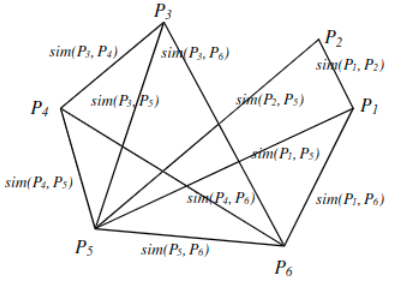
\includegraphics[width=0.5\textwidth]{lsa-trm-map.png}
    \caption{Generated TRM}
    \label{david:fig:trm-map}
\end{figure}

the "bushiness" of a node in this network is defined as the number of edges incident to that node. The top $k$ bushy sentences are arranged in order of appearance and form the summary.

\subsubsection{Similar Filtering Sentence Selection} \label{david:sec:lsa:sent-selection:similar}

One common issue with some of the methods explained above is that they may end up choosing a set of sentences that are very similar. In my modified approach, we impose a regulation parameter on Weighted Sentence Selection \ref{david:sec:lsa:sent-selection:weight}.
The specific modification to equation \ref{david:eq:weight-selection} can be seen in equation \ref{david:eq:similar-selection} where $\alpha$ is a hyper-parameter to be tuned.

\begin{equation} \label{david:eq:similar-selection}
    \text{Weight}(s_i)= \sqrt{\sum_{j=0}^n d_{ij}^2} - \left(\alpha \max_{s_j \in S/s_i} sim(s_j, s_i)\right)
\end{equation}

The results of this modified weighting scheme will be analyzed below.


\section{LSA Experiments}\label{david:sec:experiments}

We ran three different sets of experiments. The first, \ref{david:sec:experiments:similar}, looked at whether the proposed Similar Filtering Method \ref{david:sec:lsa:sent-selection:similar} is effective.
The second is an analysis of algorithms over single document sentence summarization. Finally, the same set of algorithms will be applied to multiple document summarization.

In all of the following experiments the Rouge-L metrics F-score were used to determine the comparative quality of the models.

\subsection{Similar Filtering Method Tuning}\label{david:sec:experiments:similar}

To properly evaluate the Similar Filtering Model, it was evaluated over the CNN DailyMail Dataset using TF-IDF to fill its occurrence matrix.
TF-IDF was used because the data in Tables \ref{david:table:singledoc} \& \ref{david:table:multidoc} shows that TF-IDF weighting often gave the best results. Summary lengths of $3$ were generated to obtain these results.

\begin{table}[]
    \centering
    \begin{tabular}{|l|l|}
        \hline
        Alpha                          & Score                         \\ \hline
        -0.100                         & 0.297                         \\ \hline
        \cellcolor[HTML]{F8FF00}-0.050 & \cellcolor[HTML]{F8FF00}0.301 \\ \hline
        -0.025                         & 0.301                         \\ \hline
        -0.015                         & 0.300                         \\ \hline
        0.000                          & 0.299                         \\ \hline
        0.015                          & 0.298                         \\ \hline
        0.025                          & 0.298                         \\ \hline
        0.050                          & 0.295                         \\ \hline
        0.100                          & 0.287                         \\ \hline
    \end{tabular}
    \caption{Tuning alpha parameter}
    \label{david:table:similar-alphas}
\end{table}

In Table \ref{david:table:similar-alphas}, it can be seen that the the best $\alpha = -0.050$.
Comparatively, the Weighted Method gave a F-score of $0.299$ while the Similar Filtering gave an F-score of $0.301$.

The fact the $\alpha$ parameter is negative is unintuitive, but this can be explained by the fact that summaries of sentences with high overall topic values will be similar to each other.
Therefore, a negative parameter means this method works best when emphasizing sentences that are similar to other high quality sentences.

\subsection{Single Document Summarization}\label{david:sec:experiments:singledocument}

In the following experiment, the CNN DailyMail Dataset was evaluated over the 5 methods described above (the Similar Filter Method uses an $\alpha = -0.05$) \ref{david:sec:lsa:sent-selection}. Each of these methods were then initialized with the 3 different methods of filling the occurrence matrix as defined \ref{david:sec:intro:motivation:1step}. Summaries of length $3$ were generated to obtain these results.

\begin{table}[]
    \centering
    \begin{tabular}{l l l l l l }
        \hline
                  & Naive & Weighted & Cross & Graph-Based & Similar Filter \\ \hline
        Frequency & 0.237 & 0.238    & 0.244 & 0.191       & 0.239          \\
        Binary    & 0.225 & 0.255    & 0.221 & 0.192       & 0.256          \\
        TF-IDF    & 0.256 & 0.299    & 0.257 & 0.196       & 0.301          \\
    \end{tabular}
    \caption{Single document score using F-Score of Rouge-L over the CNN DailyMail Dataset}
    \label{david:table:singledoc}
\end{table}

\subsubsection{Occurence Matrix Filling}\label{david:sec:experiments:singledocument:matrix}

In the ranking of the occurence matrix population methods, the best method was found to be the TF-IDF ranking.
For the Weighted, Similar Filtering, and Graph-Based Models, binary filling worked the second best. For the Naive and Cross Methods, using frequency worked the second best.

TF-IDF score is the most complicated metric used of the three and can encapsulate the most information. This is most likely why it performs the best.
The Frequency Method performed well for Naive and Cross Methods, because these are the simple models and can therefore use the information embedded in frequency more effectively.

\subsubsection{Model Method}\label{david:sec:experiments:singledocument:method}

Of the 5 methods, the Similar Filtering Method performs the best followed right by the Weighted Method. The Cross Method performs slightly better than the Naive Method. Finally, the Graph-Based Method performs the worst.

The Similar Filtering Method performs better than the Weighted method because it is a tuned version of the Weighted Method. The Cross Method combined more thorough approach to picking sentences hence as to why it performs better than the Naive Method.
Finally, the Graph-Based Method does comparatively not perform well. My theory is that the this method works best when dealing with large amounts of data in the $>100$ phrases range. At these document sizes, the graph component can be properly utilized better.

\subsection{Multiple Document Summarization}\label{david:sec:experiments:multidocument}

In the following experiment, the Multi-News Dataset was evaluated in the same manner as the experiment for single document summarization \ref{david:table:singledoc}. Summaries of length $10$ were generated to obtain these results.


\subsubsection{Multiple Document Modification}\label{david:sec:experiments:multidocument:modification}

To handle multiple document summarization, the summarization process was modified by including all sentences from each document in the occurrence filling matrix.

In this way, when the SVD was found, we could ensure that it was finding the most important topics across all documents.



\begin{table}
    \centering
    \begin{tabular}{l l l l l l }
        \hline
                  & Naive & Weighted & Cross & Graph-Based & Similar Filter \\ \hline
        Frequency & 0.276 & 0.273    & 0.275 & 0.205       & 0.274          \\
        Binary    & 0.269 & 0.274    & 0.266 & 0.206       & 0.273          \\
        TF-IDF    & 0.278 & 0.276    & 0.275 & 0.230       & 0.276          \\
    \end{tabular}
    \caption{Multi document score using F-Score of Rouge-L over the Multi-News Dataset}
    \label{david:table:multidoc}
\end{table}

\subsubsection{Occurence Matrix Filling}\label{david:sec:experiments:multidocument:matrix}

The most effective filling method was TF-IDF across all five selection methods, as in the Single Document Task.
The second best filling method was frequency for Naive and Cross Methods and Binary for the weight-based and graph-based methods.

The reasoning for performance is the same as in the single document case.


\subsubsection{Model Method}\label{david:sec:experiments:multidocument:method}

As in the the single document task, the performance of the classifiers is comparatively the same. This can be explained by the reasoning found in the Model Method section above \ref{david:sec:experiments:singledocument:method}.

The Graph-Based Model does perform better here and this can be attributed to the more sentences in a document caused by appending multiple documents together.

\section{Conclusions}\label{david:sec:conclusion}

LSA is an effective method of topic extraction and can be applied to the problem of extractive summarization with very few core modifications. The process in which sentences are selected is the most looked at modification within using LSA for summarization.

We have found that the most effective method is the Weighting Method. This method was slightly improved upon with the addition of adding an extra component that emphasizes similar sentences. The most effective manner for filling the occurrence matrix was using the TF-IDF value in the single document task. In the multiple document task, the most effective value for filling is the TF-IDF value as well. Better approaches can be made specifically in the area of multidocument summarization, but the naive method of appending documents together still accomplishes relatively well scoring.

\end{document}